% Options for packages loaded elsewhere
\PassOptionsToPackage{unicode}{hyperref}
\PassOptionsToPackage{hyphens}{url}
\PassOptionsToPackage{dvipsnames,svgnames,x11names}{xcolor}
%
\documentclass[
]{article}
\usepackage{amsmath,amssymb}
\usepackage{lmodern}
\usepackage{iftex}
\ifPDFTeX
  \usepackage[T1]{fontenc}
  \usepackage[utf8]{inputenc}
  \usepackage{textcomp} % provide euro and other symbols
\else % if luatex or xetex
  \usepackage{unicode-math}
  \defaultfontfeatures{Scale=MatchLowercase}
  \defaultfontfeatures[\rmfamily]{Ligatures=TeX,Scale=1}
\fi
% Use upquote if available, for straight quotes in verbatim environments
\IfFileExists{upquote.sty}{\usepackage{upquote}}{}
\IfFileExists{microtype.sty}{% use microtype if available
  \usepackage[]{microtype}
  \UseMicrotypeSet[protrusion]{basicmath} % disable protrusion for tt fonts
}{}
\makeatletter
\@ifundefined{KOMAClassName}{% if non-KOMA class
  \IfFileExists{parskip.sty}{%
    \usepackage{parskip}
  }{% else
    \setlength{\parindent}{0pt}
    \setlength{\parskip}{6pt plus 2pt minus 1pt}}
}{% if KOMA class
  \KOMAoptions{parskip=half}}
\makeatother
\usepackage{xcolor}
\usepackage{graphicx}
\makeatletter
\def\maxwidth{\ifdim\Gin@nat@width>\linewidth\linewidth\else\Gin@nat@width\fi}
\def\maxheight{\ifdim\Gin@nat@height>\textheight\textheight\else\Gin@nat@height\fi}
\makeatother
% Scale images if necessary, so that they will not overflow the page
% margins by default, and it is still possible to overwrite the defaults
% using explicit options in \includegraphics[width, height, ...]{}
\setkeys{Gin}{width=\maxwidth,height=\maxheight,keepaspectratio}
% Set default figure placement to htbp
\makeatletter
\def\fps@figure{htbp}
\makeatother
\setlength{\emergencystretch}{3em} % prevent overfull lines
\providecommand{\tightlist}{%
  \setlength{\itemsep}{0pt}\setlength{\parskip}{0pt}}
\setcounter{secnumdepth}{-\maxdimen} % remove section numbering
% definitions for citeproc citations
\NewDocumentCommand\citeproctext{}{}
\NewDocumentCommand\citeproc{mm}{%
  \begingroup\def\citeproctext{#2}\cite{#1}\endgroup}
\makeatletter
 % allow citations to break across lines
 \let\@cite@ofmt\@firstofone
 % avoid brackets around text for \cite:
 \def\@biblabel#1{}
 \def\@cite#1#2{{#1\if@tempswa , #2\fi}}
\makeatother
\newlength{\cslhangindent}
\setlength{\cslhangindent}{1.5em}
\newlength{\csllabelwidth}
\setlength{\csllabelwidth}{3em}
\newenvironment{CSLReferences}[2] % #1 hanging-indent, #2 entry-spacing
 {\begin{list}{}{%
  \setlength{\itemindent}{0pt}
  \setlength{\leftmargin}{0pt}
  \setlength{\parsep}{0pt}
  % turn on hanging indent if param 1 is 1
  \ifodd #1
   \setlength{\leftmargin}{\cslhangindent}
   \setlength{\itemindent}{-1\cslhangindent}
  \fi
  % set entry spacing
  \setlength{\itemsep}{#2\baselineskip}}}
 {\end{list}}
\usepackage{calc}
\newcommand{\CSLBlock}[1]{\hfill\break\parbox[t]{\linewidth}{\strut\ignorespaces#1\strut}}
\newcommand{\CSLLeftMargin}[1]{\parbox[t]{\csllabelwidth}{\strut#1\strut}}
\newcommand{\CSLRightInline}[1]{\parbox[t]{\linewidth - \csllabelwidth}{\strut#1\strut}}
\newcommand{\CSLIndent}[1]{\hspace{\cslhangindent}#1}
\ifLuaTeX
\usepackage[bidi=basic]{babel}
\else
\usepackage[bidi=default]{babel}
\fi
\babelprovide[main,import]{american}
% get rid of language-specific shorthands (see #6817):
\let\LanguageShortHands\languageshorthands
\def\languageshorthands#1{}
\ifLuaTeX
  \usepackage{selnolig}  % disable illegal ligatures
\fi
\IfFileExists{bookmark.sty}{\usepackage{bookmark}}{\usepackage{hyperref}}
\IfFileExists{xurl.sty}{\usepackage{xurl}}{} % add URL line breaks if available
\urlstyle{same} % disable monospaced font for URLs
\hypersetup{
  pdftitle={genomesizeR: An R package for genome size prediction},
  pdfauthor={Celine Mercier, Joane Elleouet},
  pdflang={en-US},
  colorlinks=true,
  linkcolor={Maroon},
  filecolor={Maroon},
  citecolor={Blue},
  urlcolor={Blue},
  pdfcreator={LaTeX via pandoc}}

\title{genomesizeR: An R package for genome size prediction}

%%%%%%%%%%%%%%%%%%%%%%%%%%%%%%%%%%%%%%%%%%%%%%%%%%%%%%%%%%%%%%%%%%%%%%%%
% Authors and Affiliations

\usepackage[affil-it]{authblk}
\usepackage{orcidlink}
%% \renewcommand\Authsep{, }
\setlength{\affilsep}{1em}
\author[1%
  *%
  ]{Celine Mercier%
    \,\orcidlink{0000-0002-4782-1530}\,%
    }
\author[1%
  *%
  ]{Joane Elleouet%
    \,\orcidlink{0000-0002-9597-3360}\,%
    }

\affil[1]{Scion, New Zealand Forest Research Institute, New Zealand}
\affil[*]{These authors contributed equally.}
%%%%%%%%%%%%%%%%%%%%%%%%%%%%%%%%%%%%%%%%%%%%%%%%%%%%%%%%%%%%%%%%%%%%%%%%
\date{14 June 2024}

\begin{document}
\maketitle

\section{Summary}\label{summary}

The genome size of organisms present in an environment can provide many
insights into evolutionary and ecological processes at play in that
environment. The genomic revolution has enabled a rapid expansion of our
knowledge of genomes in many living organisms, and most of that
knowledge is classified and readily available in the databases of the
National Center for Biotechnology Information (NCBI). The
\texttt{genomesizeR} tool leverages the wealth of taxonomic and genomic
information present in NCBI databases to infer the genome size of
Archeae, Bacteria, or Eukaryote organisms identified at any taxonomic
level. This R package uses statistical modelling on data from the most
up-to-date NCBI databases and provides three statistical methods for
genome size prediction of a given taxon, or group of taxa. A
straightforward `weighted mean' method identifies the closest taxa with
available genome size information in the taxonomic tree, and averages
their genome sizes using weights based on taxonomic distance. A
frequentist random effect model uses nested genus and family information
to output genome size estimates. Finally a third option provides
predictions from a distributional Bayesian multilevel model which uses
taxonomic information from genus all the way to superkingdom, therefore
providing estimates and uncertainty bounds even for under-represented
taxa.

All three methods use:

\begin{itemize}
\tightlist
\item
  A list of queries; a query being a taxon or a list of several taxa.
  The package was designed to make it easy to use with data coming from
  environmental DNA experiments, but works with any table of taxa.
\item
  A reference database containing all the known genome sizes, built from
  the NCBI databases, with associated taxa, provided in an archive to
  download.
\item
  A taxonomic tree structure as built by the NCBI, provided in the same
  archive.
\end{itemize}

\texttt{genomesizeR} retrieves the taxonomic classification of input
queries, estimates the genome size of each query, and provides 95\%
confidence intervals for each estimate.

\section{Statement of need}\label{statement-of-need}

The size of microbial genomes and its evolution can provide important
insights into evolutionary and ecological processes influencing both
microbial species and the environments in which they inhabit. The
shedding of unnecessary genetic elements and their associated
biosynthetic pathways, for example, is a common phenomenon observed in
organisms with a high degree of host symbiosis
(\citeproc{ref-brader2014metabolic}{Brader et al., 2014};
\citeproc{ref-moran2002microbial}{Moran, 2002};
\citeproc{ref-vandenkoornhuyse2007active}{Vandenkoornhuyse et al.,
2007}). Genome size reduction has also been observed in organisms
experiencing arid environments (\citeproc{ref-liu2023warmer}{Liu et al.,
2023}), or a narrow range of substrates or metabolic options
(\citeproc{ref-tyson2004community}{Tyson et al., 2004}). Among many
others, these findings demonstrate the opportunities associated with
including genome size as a key trait in microbial communities to provide
insights spanning niche size, co-evolution, adaption, and metabolic
flexibility of the microbiomes present, but also stability, and
ecophysiological and functional complexity of abiotic and biotic
environments.

However, characterizing genome size for all organisms in a microbiome
remains challenging. Methods in the past have included the use of DNA
staining through to cell enumeration, flow cytometry, culturing, gel
electrophoresis, and DNA renaturation kinetics. All have merits and
limitations (\citeproc{ref-raes2007prediction}{Raes et al., 2007}). The
widespread availability and use of microbiome related tag-amplicon DNA
sequencing has tremendously increased our scientific knowledge of
microbial genomics. There is also an opportunity to explore the rapidly
expanding archives of short read DNA libraries (i.e.~extant 16S and ITS
amplicon sequences).

Alternatively, when well documented and archived in user-friendly and
publicly available databases, the exponentially growing genomic
knowledge of micro-organisms is an inexpensive resource unlocking a
myriad of research opportunities in all fields of environmental
sciences, from human and agricultural microbiomes through to aquatic,
soil, and atmospheric ecosystems. Combining available genome size
information to data and metadata on community structure from existing
projects can add further scientific value to investment already made in
these projects, at no added cost.

However, genome size estimates for many taxa found in environmental
samples are missing from public databases, or fully unknown. The
evolutionary rule that phylogenetically related organisms share genetic
similarities can be exploited and genome size for taxa with unknown
genome size can be statistically inferred from related taxa with known
genome size, using taxonomy as a proxy for phylogeny. Another challenge
is the precision of identification: some taxa can only be identified at
high taxonomic levels. Statistical methods can also be used to infer
their genome size range from databases. To our knowledge, there is no
convenient and fast way to obtain genome size estimates with uncertainty
bounds for all organisms identified or partially identified in an
environmental sample.

Using the increased prevalence of whole-genome information for all
organisms, we have therefore developed \texttt{genomesizeR}, allowing
the inference of genome size of many queries at once, based on taxonomic
information and available genome data from the National Center for
Biotechnology Information (NCBI).

\section{Methods}\label{methods}

\subsection{NCBI database filtering and
processing}\label{ncbi-database-filtering-and-processing}

The reference database used is built by querying all genome metadata
information from the curated NCBI RefSeq database
(\citeproc{ref-OLeary2016-kw}{O'Leary et al., 2016}). Filters are
applied to only keep full genomes, and discard data that the NCBI has
tagged as anomalous, or abnormally large or small.

This raw database is then prepared to include more pre-computed
information to be used by the package. Genome sizes are aggregated to
the species level by iteratively averaging all entries below, hence the
package can only provide estimates at the level of species and above.
Average genome sizes and their associated standard error values are also
pre-computed, to be used by the weighted mean method.

\subsection{Bayesian method}\label{bayesian-method}

The NCBI database of species with known genome sizes was split by
superkingdom (Bacteria, Archeae, Eukaryotes). A distributional Bayesian
linear hierarchical model using the \texttt{brm} function from the
\texttt{brms} package was fitted to each superkingdom dataset. The
general model structure is outlined below.

\begin{gather*}
log(G_i) \sim \mathcal{N}(\mu_i, \sigma_{i}^2)
\end{gather*}

where \(G_i\) is the genome size of species \(i\) in the units of 10
Mbp. The model uses predictors for both mean and standard deviation. The
mean is modelled as follows:

\begin{gather*}
\mu_i = \alpha_0 + \alpha_{genus_{g[i]}} + \alpha_{family_{f[i]}} + \alpha_{order_{o[i]}} + \alpha_{class_{c[i]}} + \alpha_{phylum_{p[i]}}  \\
\alpha_{genus_{g[i]}} \sim \mathcal{N}(0, \sigma_{genus}^2) \\
\alpha_{family_{f[i]}} \sim \mathcal{N}(0, \sigma_{family}^2) \\
\alpha_{order_{o[i]}} \sim \mathcal{N}(0, \sigma_{order}^2) \\
\alpha_{class_{c[i]}} \sim \mathcal{N}(0, \sigma_{class}^2) \\
\alpha_{phylum_{p[i]}} \sim \mathcal{N}(0, \sigma_{phylum}^2) \\
\end{gather*}

The following prior distributions are used:

\begin{gather*}
\alpha_0 \sim \mathcal{N}(0,5) \\
(\sigma_{genus},\sigma_{family},\sigma_{order},\sigma_{class},\sigma_{phylum},s_{class},s_{phylum}) \sim \mathcal{N}^+(0,1) \\
\end{gather*}

Differences in genome size variability was observed among taxa,
therefore the model also adds predictors to the standard deviation of
the response. The standard deviation is modelled as follows:

\begin{gather*}
log(\sigma_{i}) = \lambda_0 + \lambda_{class_{c[i]}} + \lambda_{phylum_{p[i]}} \\
\lambda_{class_{c[i]}} \sim \mathcal{N}(0, s_{class}^2) \\
\lambda_{phylum_{p[i]}} \sim \mathcal{N}(0, s_{phylum}^2) \\
\end{gather*}

with priors

\begin{gather*}
\lambda_0 \sim \mathcal{N}(0,1) \\
(s_{class},s_{phylum}) \sim \mathcal{N}^+(0,1) \\
\end{gather*}

\(\mathcal{N}^+\) is the normal distribution truncated to positive
values. \(g[i]\),\(f[i]\),\(o[i]\),\(c[i]\) and \(p[i]\) are
respectively the index for the genus, family, order, class, and phylum
of entry \(i\) in the species-level database. Note that taxonomic groups
are naturally nested within each other and the indices are designed to
be unique to the particular taxonomic group it represents.

The estimation process uses Stan's Hamiltonian Monte Carlo algorithm
with the U-turn sampler.

Posterior predictions are obtained using the \texttt{predict} function
from the \texttt{brms} package, and 95\% credible intervals are obtained
using 2.5\% and 97.5\% quantiles from the posterior distribution.

Queries corresponding to identified species with an available genome
size estimate in the NCBI database get allocated the genome size value
of the database (averaged at the species level) and 95\% confidence
intervals are calculated as XXX

\subsection{Frequentist method}\label{frequentist-method}

A frequentist linear mixed-effects model using the \texttt{lmer}
function from the \texttt{lme4} package
(\citeproc{ref-bates2015lme4}{Bates et al., 2015}) was fitted to the
NCBI database of species with known genome sizes. The model is as
follows:

\begin{gather*}
log(G_i) =  \alpha_0 + \alpha_{genus_{g[i]}} +  \alpha_{family_{f[i]}} + e_i \\
\end{gather*} where \(\alpha_0\) is the overall mean,
\(\alpha_{genus_{g[i]}}\) and \(\alpha_{family_{f[i]}}\) are random
effect of genus and family for genus \(g[i]\) and family \(f[i]\) and
\(e_i\) is the residual error of observation \(i\).

The estimation process using the restricted maximum likelihood method
(REML). A prediction interval is computed using the
\texttt{predictInterval} function from the \texttt{merTools} package
(\citeproc{ref-knowles2024mertools}{Knowles \& Frederick, 2024}). As
higher nested levels (order, class) are not taken into account in the
model, predictions are not produced for queries above the family level.

\subsection{Weighted mean method}\label{weighted-mean-method}

The weighted mean method computes the genome size of a query by
averaging the known genome sizes of surrounding taxa in the taxonomic
tree, with a weighted system where further neighbours have less weight
in the computed mean. The identification of related taxa is limited to
levels below and including order.

In the calculation of the prediction for a given query, the weight for a
related taxon in the database is calculated as

\begin{gather*}
w_i = \frac{1}{d_i + 1}
\end{gather*}

where \(d_i\) is the distance of the related taxon to the query in
number of nodes in the taxonomy.

The confidence interval is calculated as:

\begin{equation}
CI = 1.96 \times \sqrt{\hat{\mu}}
\end{equation}

where \(\hat{\mu}\) is the computed weighted mean.

For queries relating to well-characterised species where many genetic
studies have been performed, such as model organisms, this might lead to
more precise predictions than the two other methods. This method can
also perform better than the others if your queries consist of lists of
taxa (for example, an output of \emph{blastn} where several matches can
be obtained for each query). Otherwise, we suggest using one of the
other methods, as the confidence intervals calculated are less reliable
for the weighted mean method.

\section{Implementation}\label{implementation}

The main steps of all methods are multithreaded on POSIX systems using
the packages parallel (\citeproc{ref-R2024}{R Core Team, 2024}) and
doParallel (\citeproc{ref-weston2022doparallel}{Corporation \& Weston,
2022}).

The packages ncbitax (\citeproc{ref-ncbitax2020}{Machne, 2022}) and
CHNOSZ (\citeproc{ref-Dick2019-nl}{Dick, 2019}) are used to read the
taxonomy data, dplyr (\citeproc{ref-dplyr2023}{Wickham et al., 2023})
and biomformat (\citeproc{ref-biomformat2024}{McMurdie \& Paulson,
2024}) are used for some of the formatting, and pbapply
(\citeproc{ref-pbapply2023}{Solymos \& Zawadzki, 2023}) is used to
display the progress bar.

The R package accepts as input formats the common `taxonomy table'
format used by popular packages such as phyloseq
(\citeproc{ref-phyloseq2013}{McMurdie \& Holmes, 2013}) and mothur
(\citeproc{ref-schloss_introducting_2009}{Schloss et al., 2009}), and
any file or data frame with a column containing either NCBI taxids or
taxon names. The output format is a data frame with the same columns as
the input, with some added columns providing information about the
estimation and the quality of the estimation. The user can also choose a
simple output format only containing the estimation information.

Several plotting functions using the ggplot2
(\citeproc{ref-ggplot22016}{Wickham, 2016}) and ggtree
(\citeproc{ref-Yu2020-pa}{Yu, 2020}) packages are also provided to
visualise the results.

\section{Method comparison}\label{method-comparison}

The applicability of each method varies. The Bayesian method outputs
results for any taxon that is recognised in the NCBI taxonomy. The
frequentist random effects model method only outputs results for queries
that have a match at the species, genus, or family level. The weighted
mean method only performs an estimation for queries that have at least
two matches at the species, genus, family, or order level. Below is a
comparison of estimates for an example set of bacteria and fungi queries
where the highest level of match with the database is the family level.
Note that there are fewer successful estimations with the weighted mean
method than with the two model-based methods.

Figures below show that estimates and the width of confidence intervals
differ between methods (figures \autoref{fig:est_comp},
\autoref{fig:CI_comp} and \autoref{fig:CI_rel_comp}).

\begin{figure}
\centering
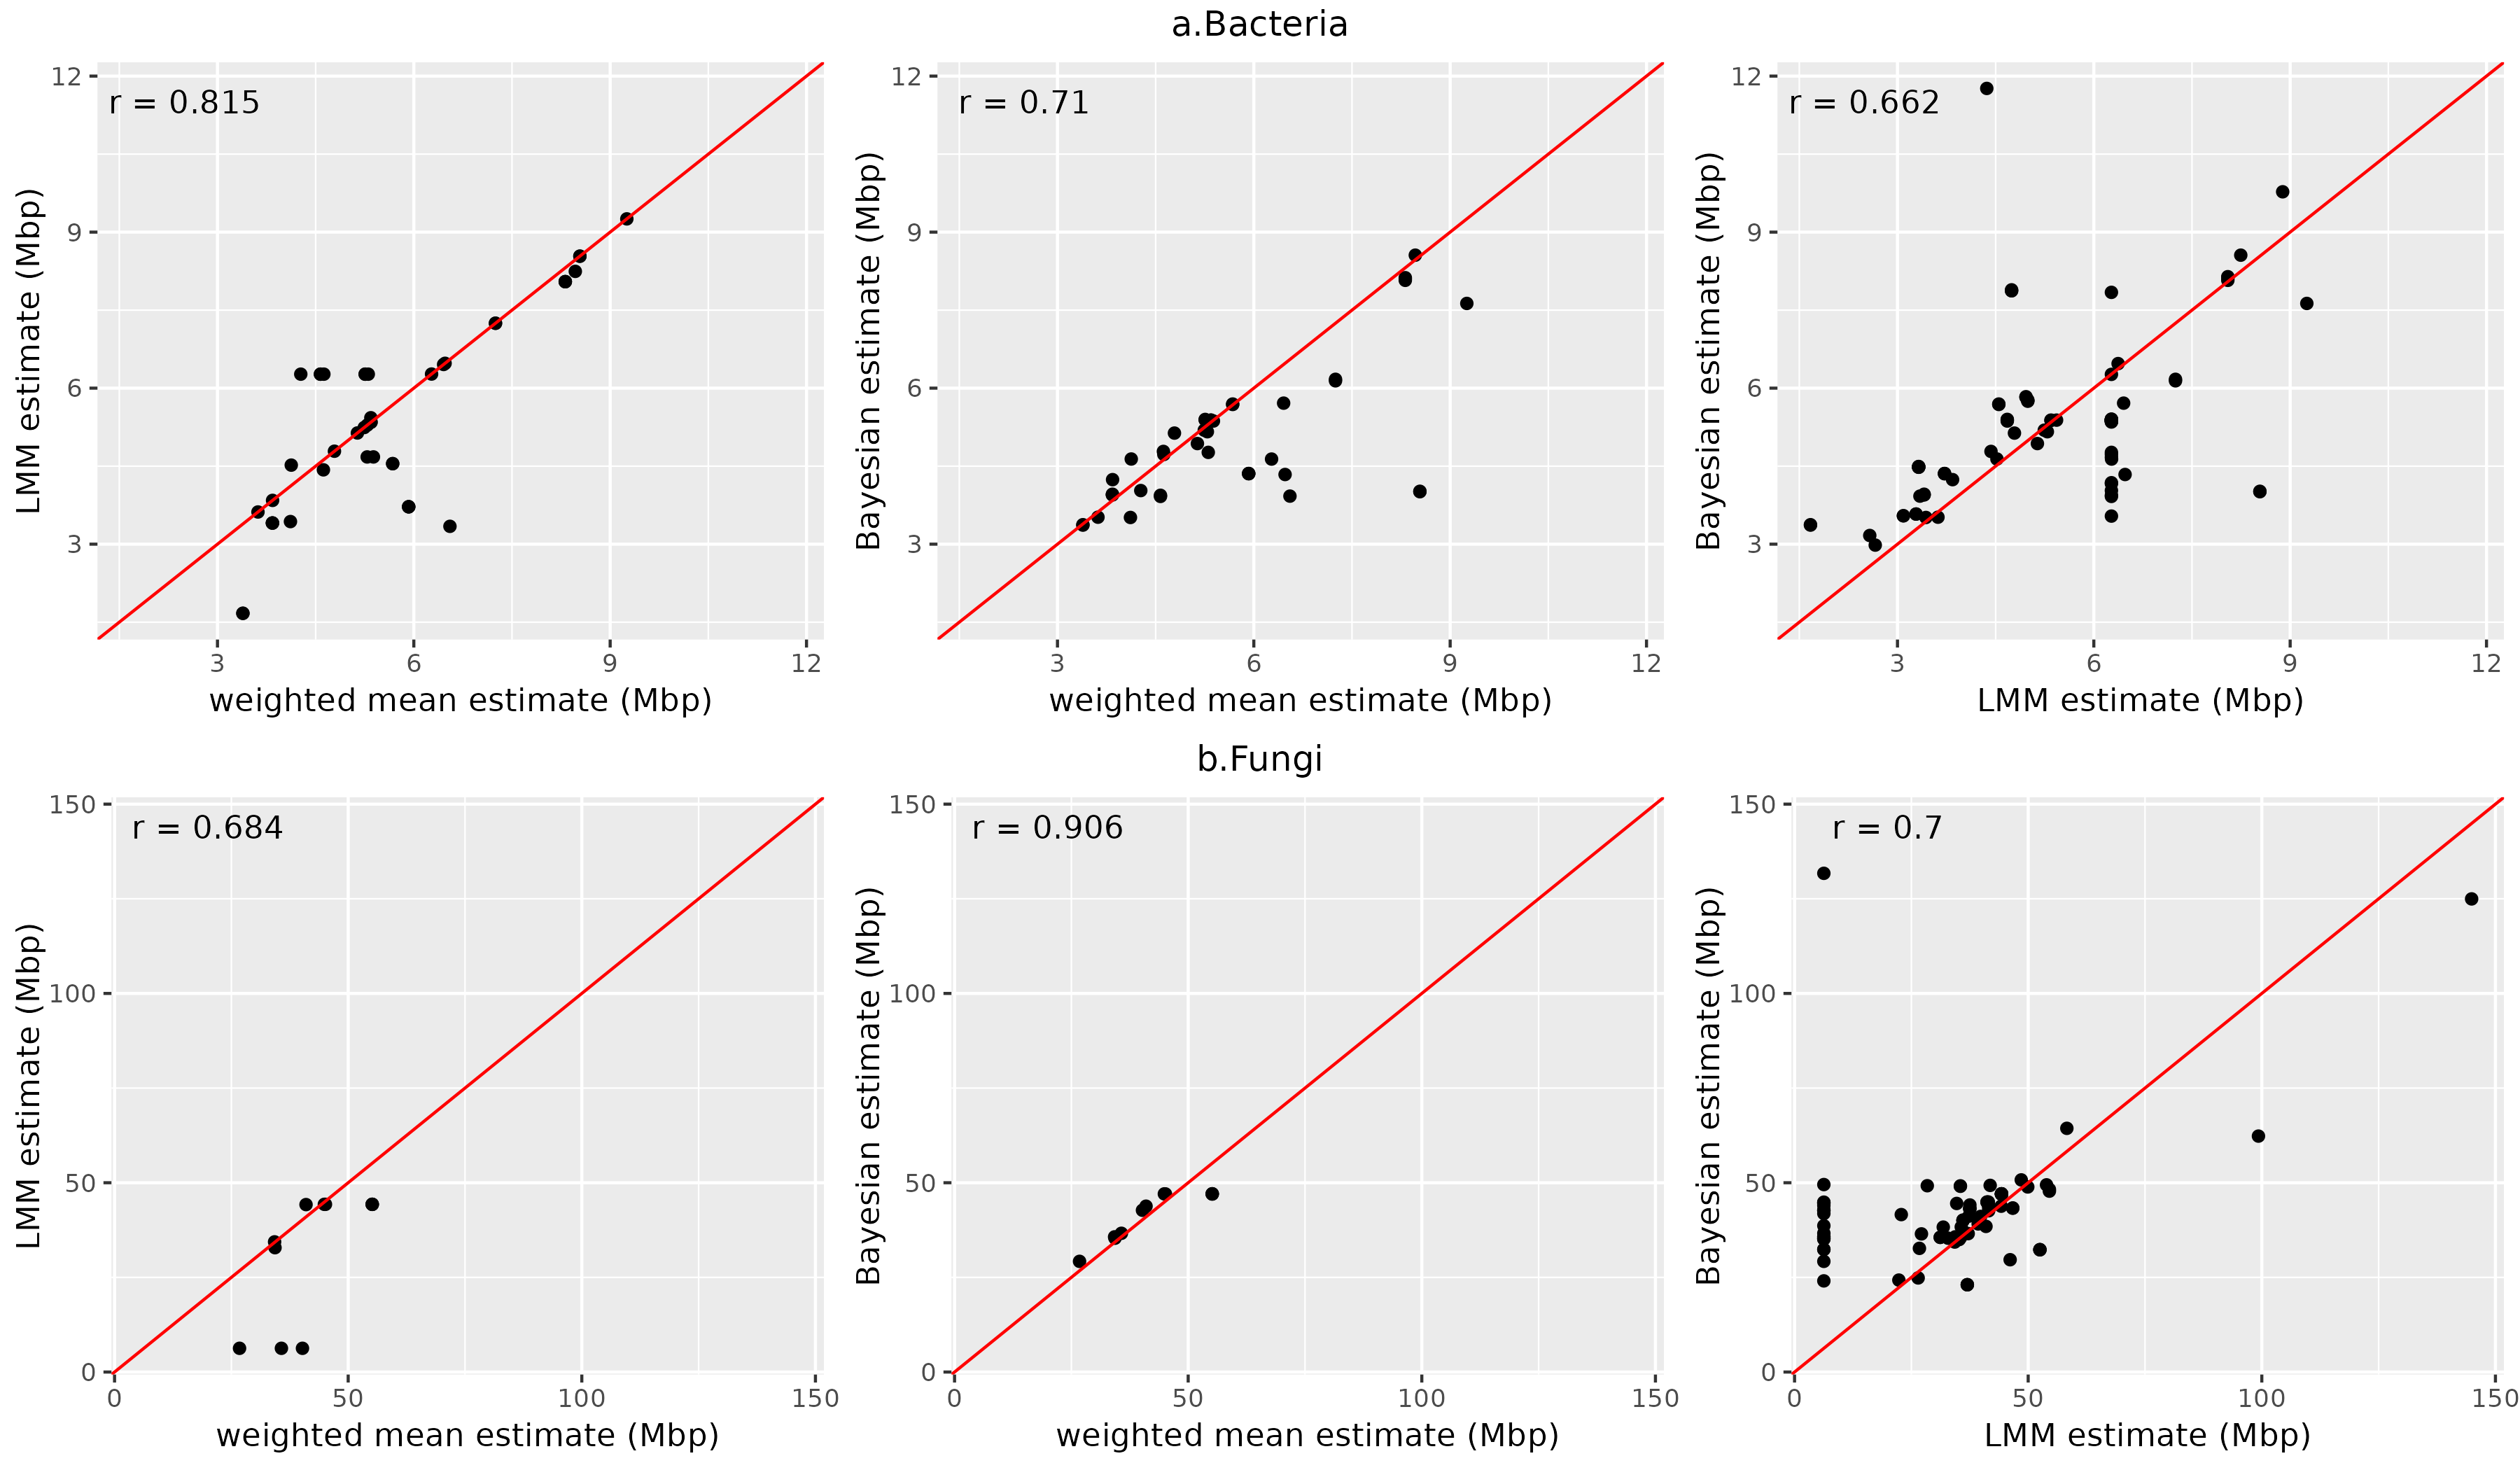
\includegraphics[width=1\textwidth,height=\textheight]{compare_estimates.png}
\caption{Pairwise comparison of estimates from different methods for a.
bacteria and b. fungi. Pearson's correlation coefficient is displayed at
the top left.\label{fig:est_comp}}
\end{figure}

\begin{figure}
\centering
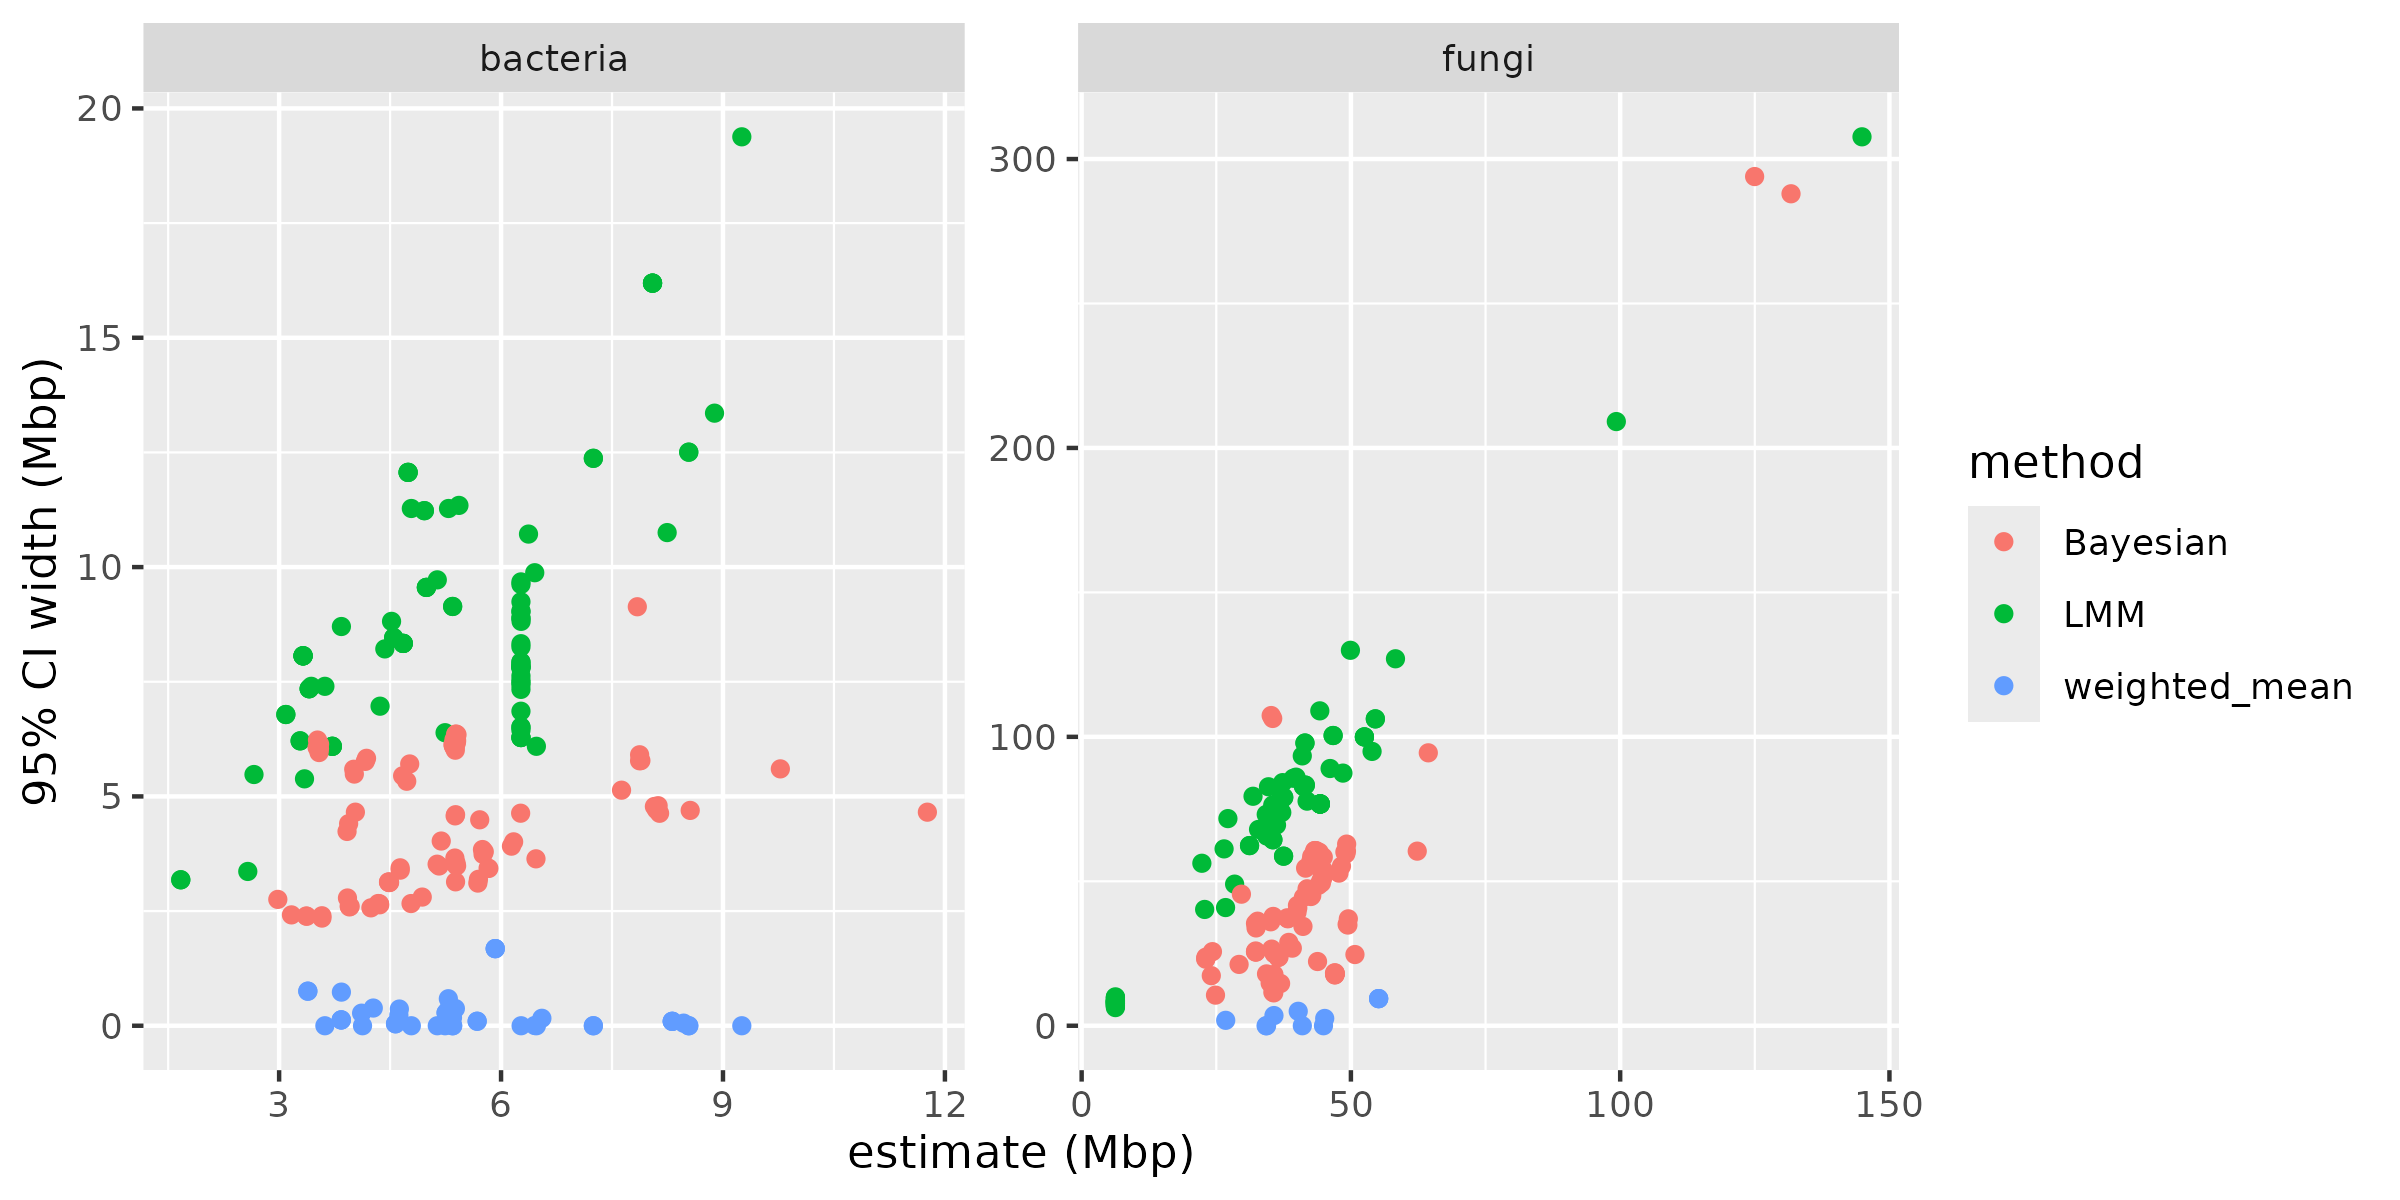
\includegraphics[width=0.75\textwidth,height=\textheight]{compare_CI.png}
\caption{Pairwise comparison of 95\% confidence intervals from different
methods for a. bacteria and b. fungi.\label{fig:CI_comp}}
\end{figure}

\begin{figure}
\centering
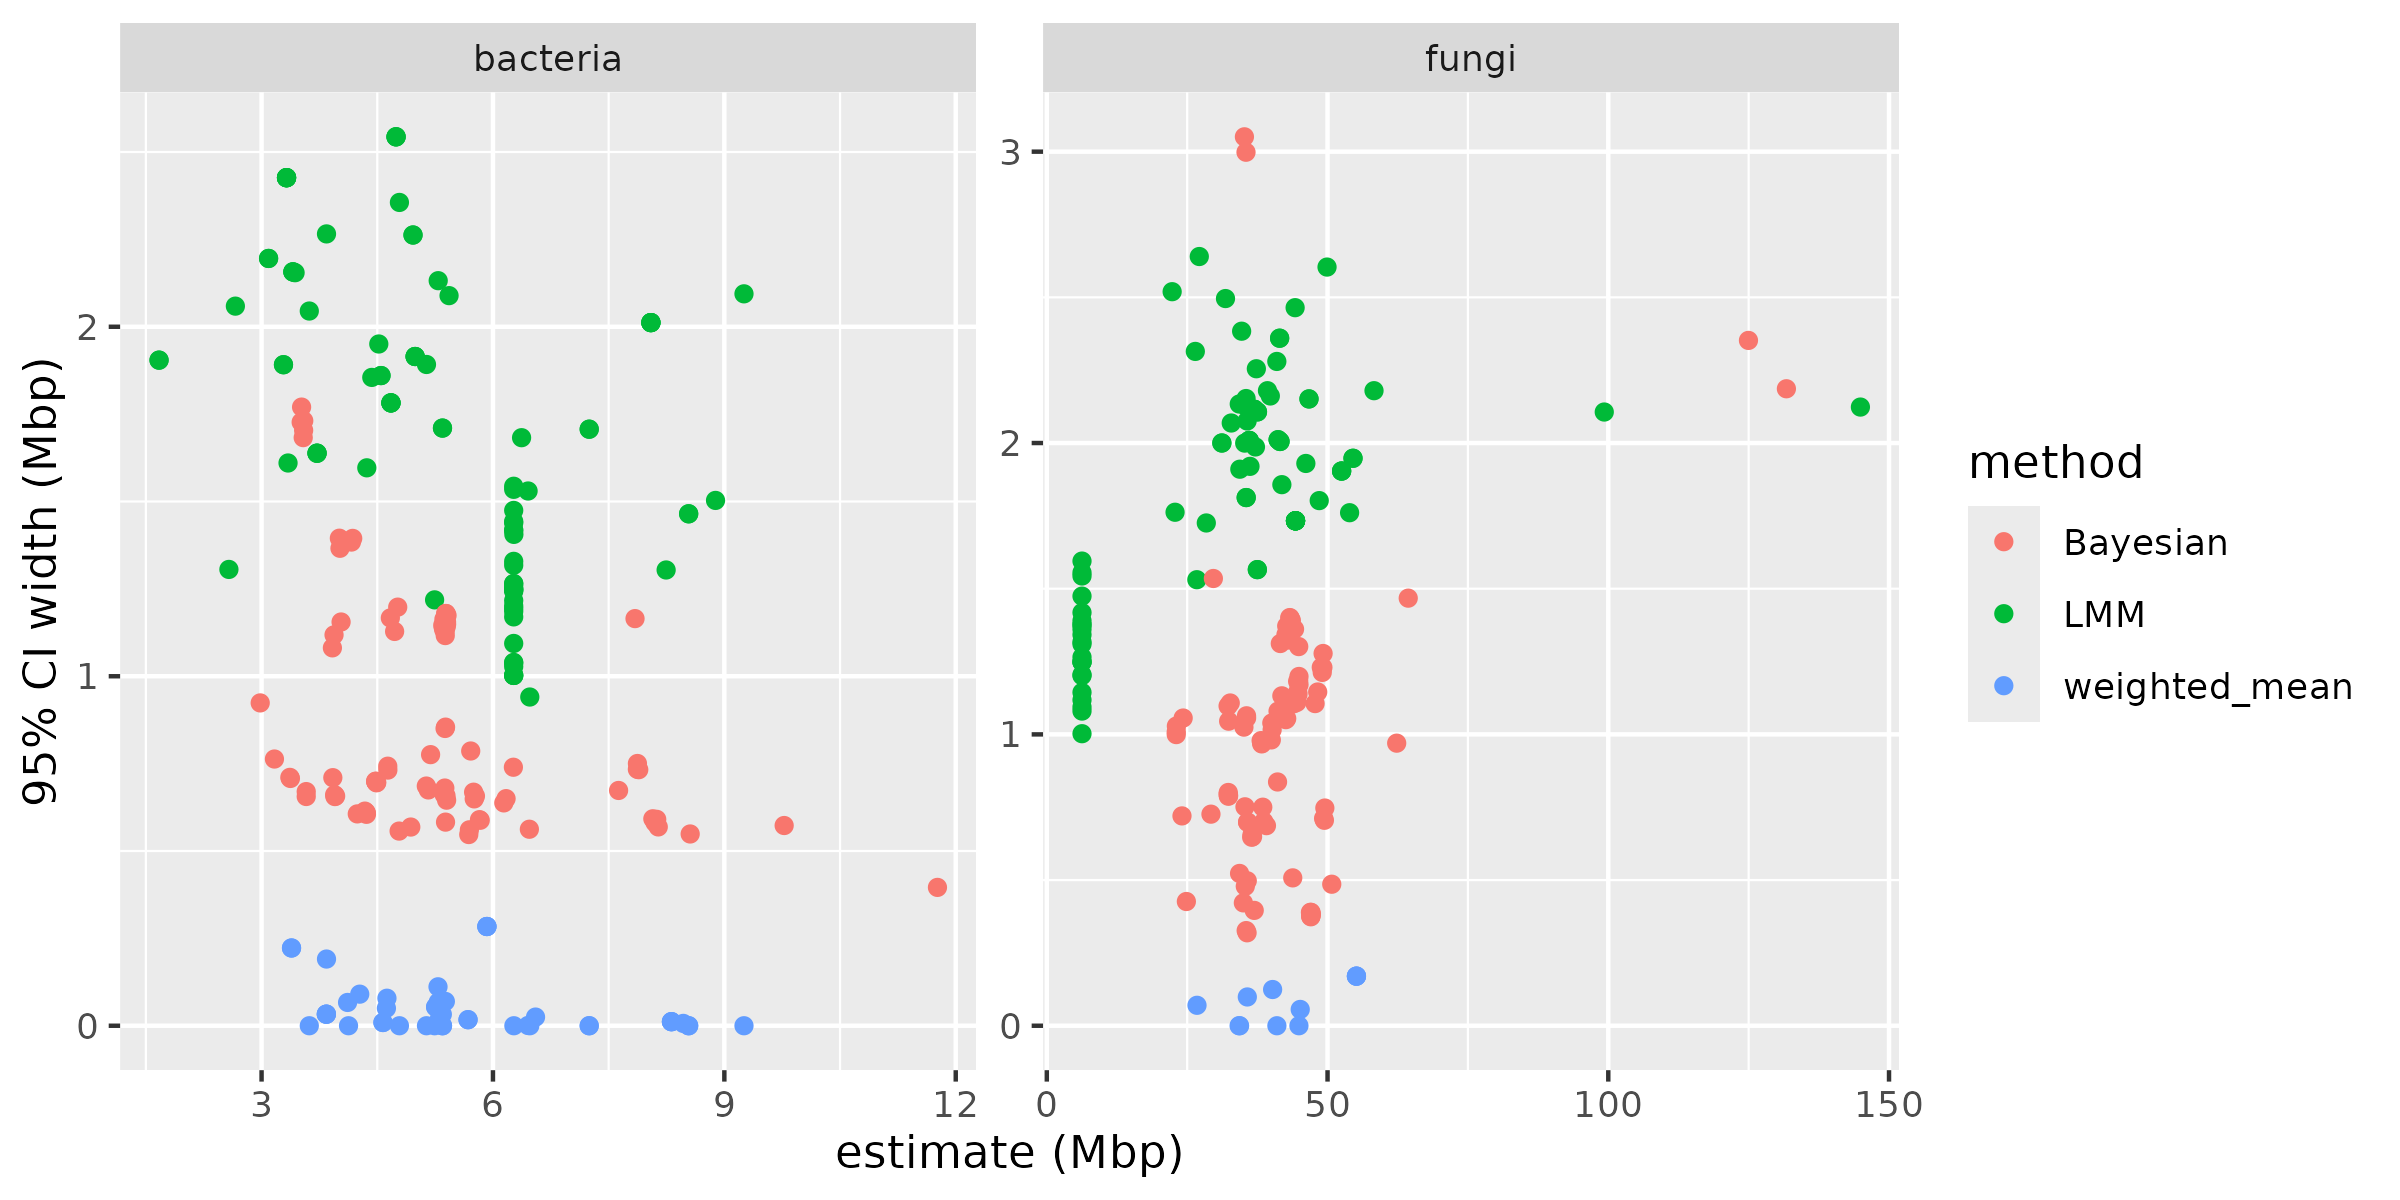
\includegraphics[width=0.75\textwidth,height=\textheight]{compare_CI_rel.png}
\caption{Pairwise comparison of relative 95\% confidence intervals
(scaled by estimated size) from different methods for a.bacteria and
b.fungi.\label{fig:CI_rel_comp}}
\end{figure}

\section{Example}\label{example}

This example data is a subset of the dataset from Labouyrie et al.
(\citeproc{ref-Labouyrie2023-yc}{2023}).

First, the genome sizes are predicted from the taxa:

\texttt{results\ =\ estimate\_genome\_size(example\_input\_file,\ refdata\_archive\_path,\ sep=\textquotesingle{}\textbackslash{}t\textquotesingle{},\ match\_column=\textquotesingle{}TAXID\textquotesingle{},\ output\_format=\textquotesingle{}input\textquotesingle{})}

\begin{verbatim}
#############################################################################
# Genome size estimation summary:
#
#  32.22222 % estimations achieving required precision
#
     Min.   1st Qu.    Median      Mean   3rd Qu.      Max. 
  2260662   4850009  15733757  23739845  39882934 161191581 

# Estimation status:
Confidence interval to estimated size ratio > ci_threshold  | OK 
                                                       122  | 58 
\end{verbatim}

Then, the results can be visualized using the plotting functions
provided. \autoref{fig:example_hist_box} shows a histogram and a boxplot
of the estimated genome sizes for each sample.
\autoref{fig:example_tree} shows a tree showing the taxonomic
relationships as well as the estimated genome sizes.

\begin{figure}
\centering
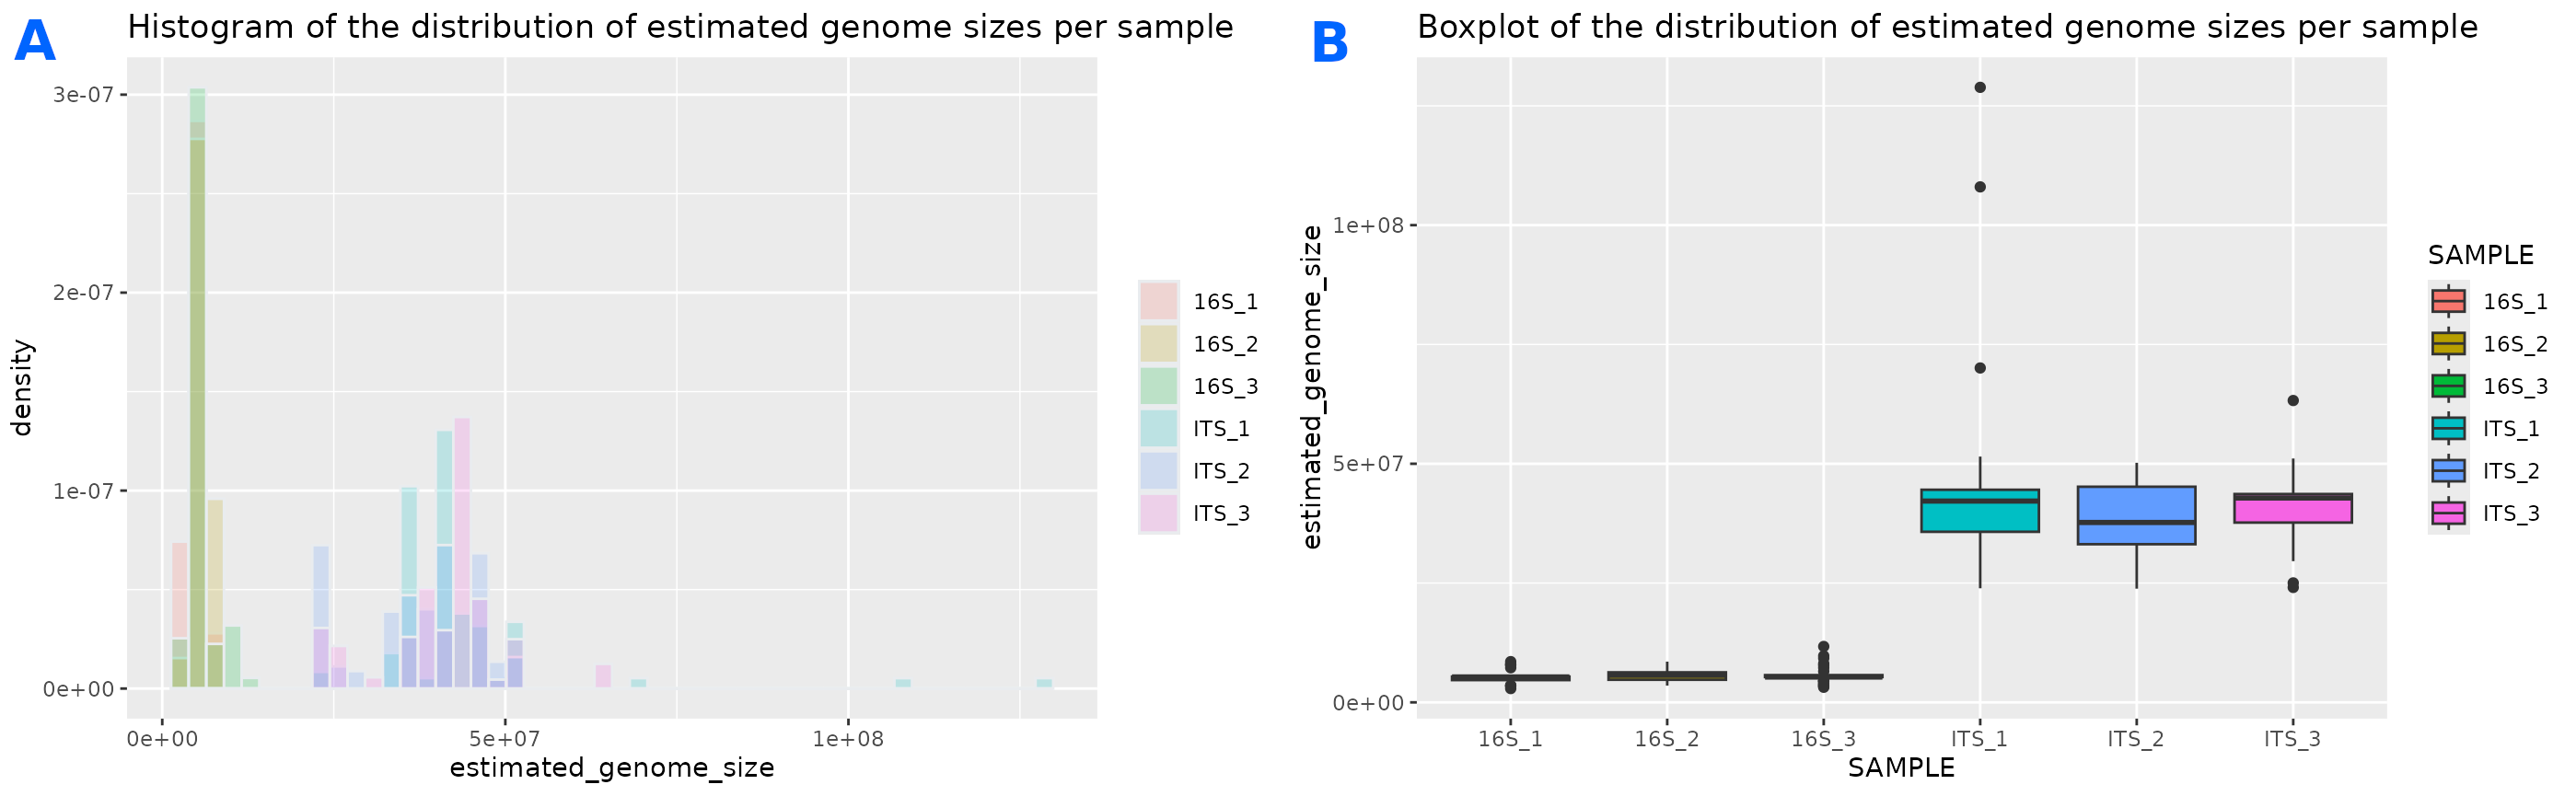
\includegraphics[width=1\textwidth,height=\textheight]{example_hist_boxplot.png}
\caption{Histogram (A) and boxplot (B) of estimated genome sizes for
each sample\label{fig:example_hist_box}}
\end{figure}

\begin{figure}
\centering
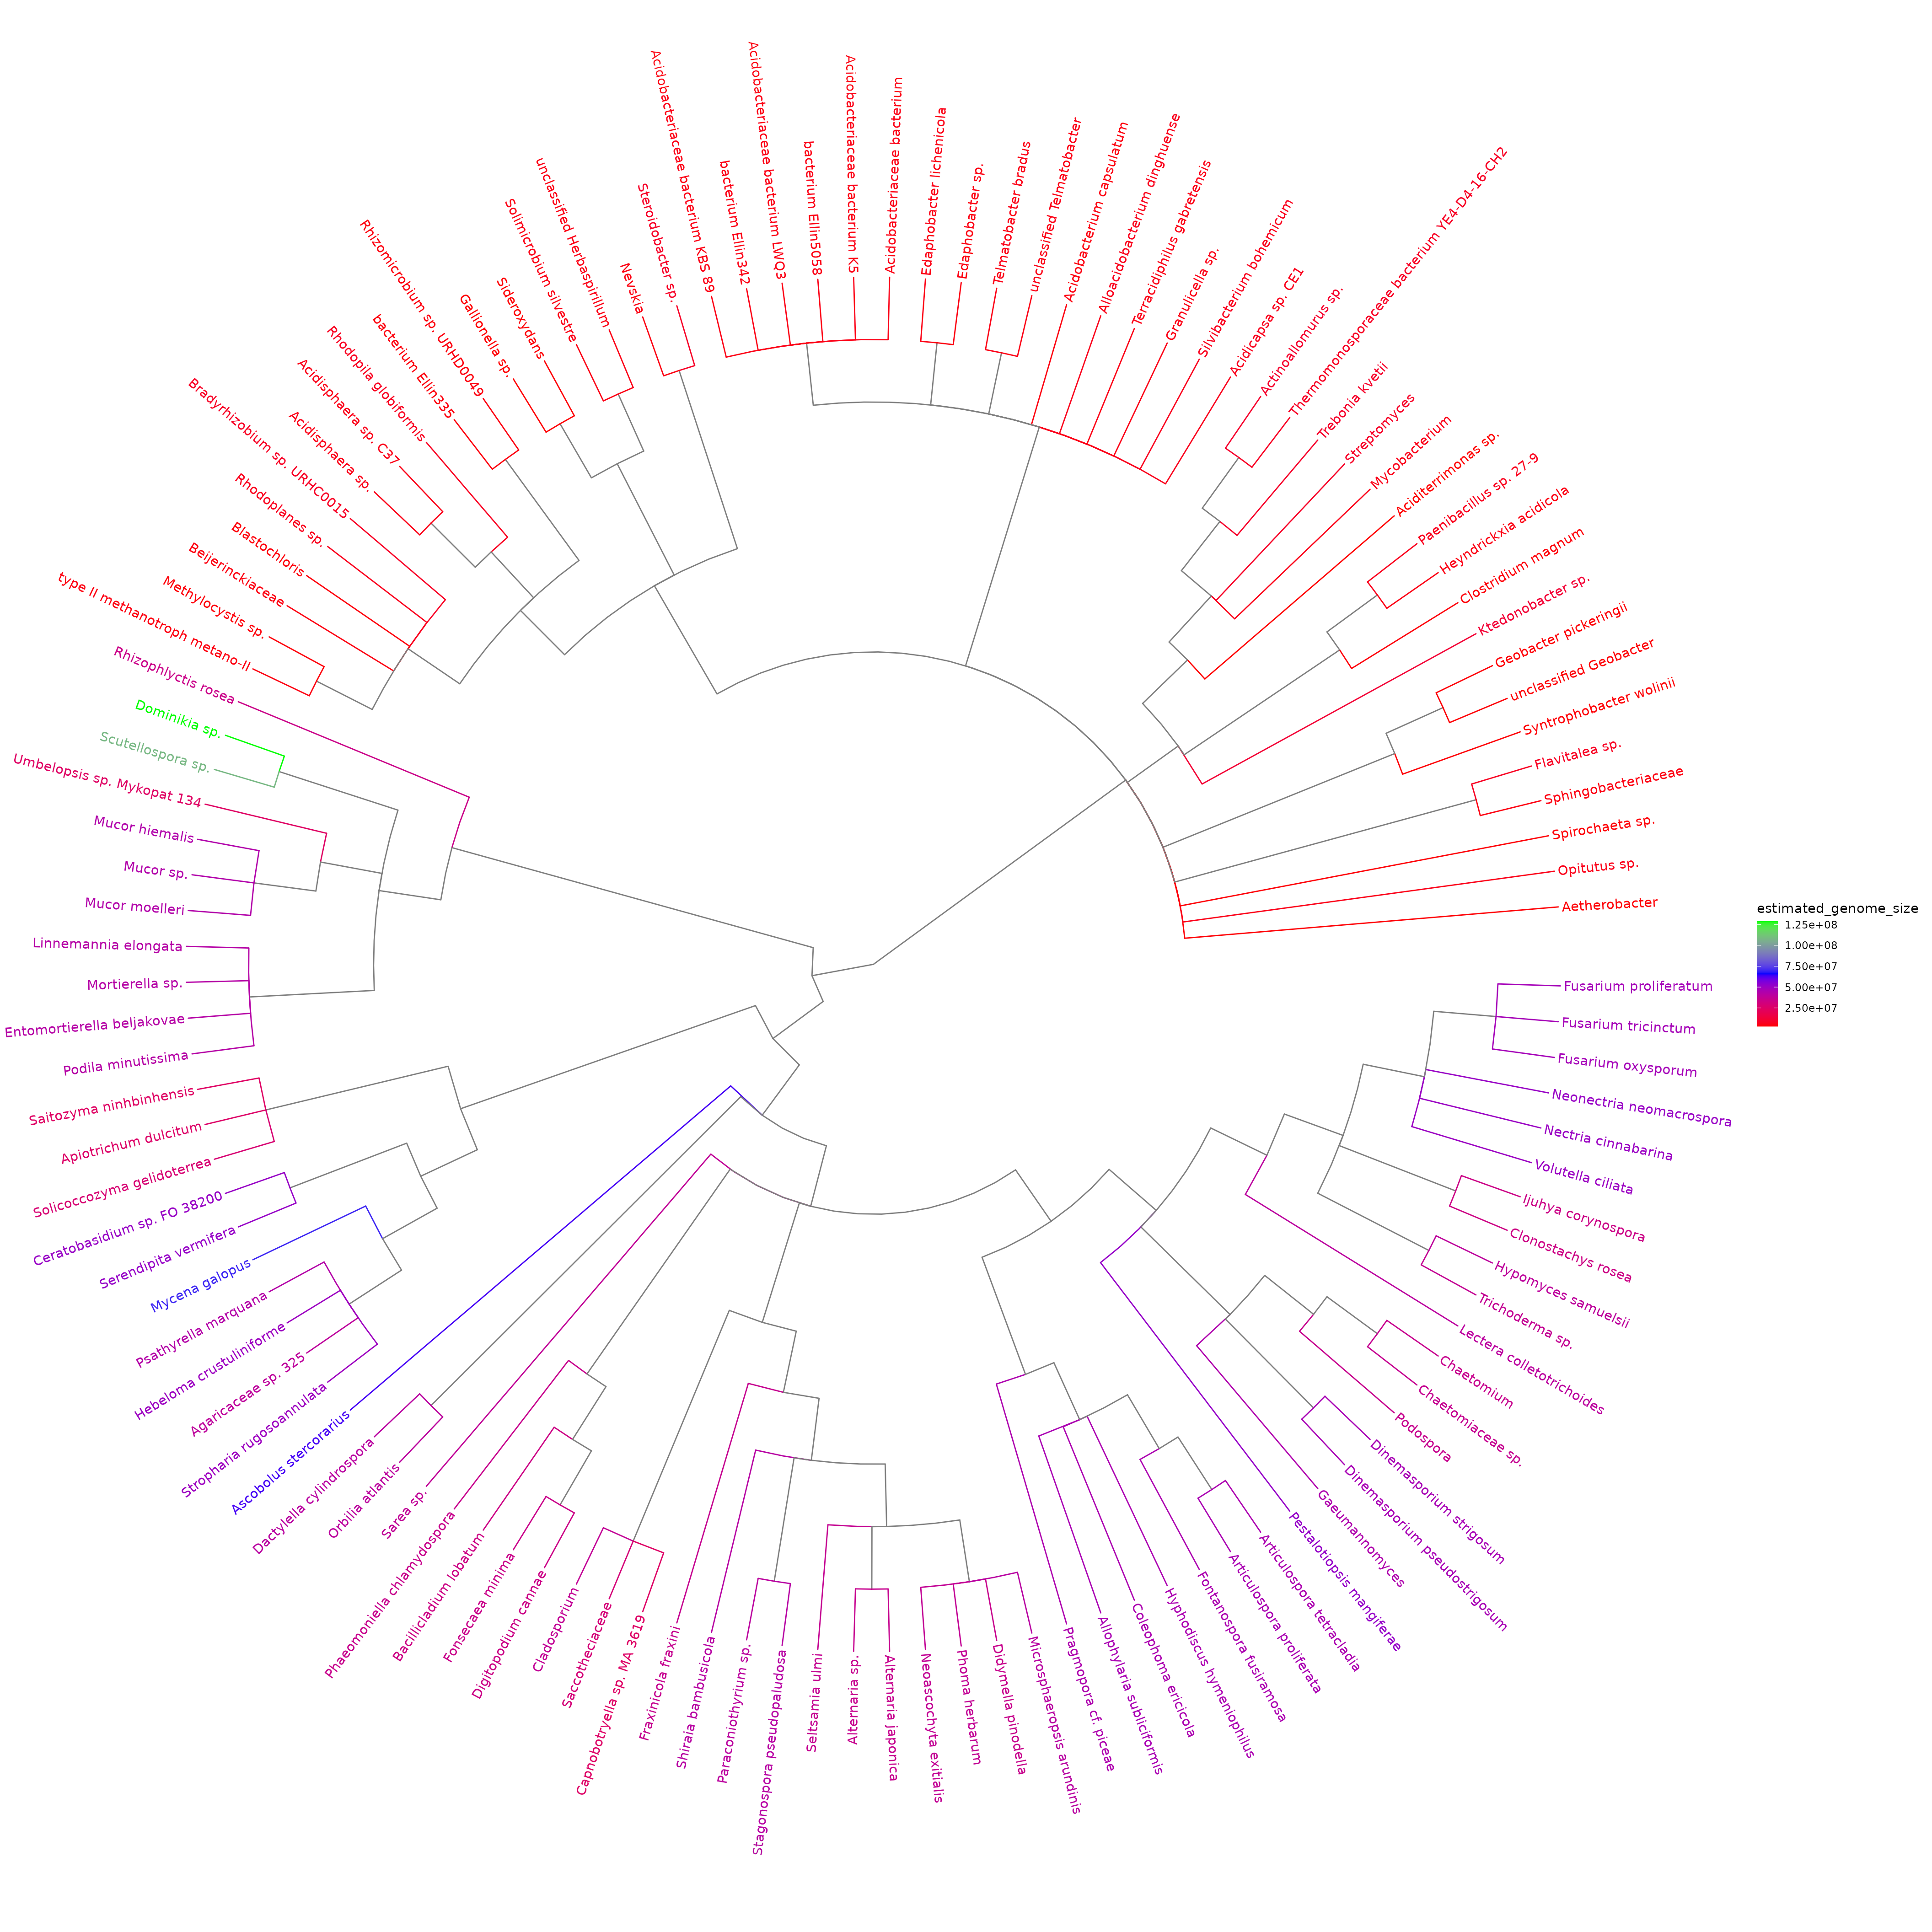
\includegraphics[width=1\textwidth,height=\textheight]{example_tree.png}
\caption{Tree representing taxonomic relationships and estimated genome
sizes between queries\label{fig:example_tree}}
\end{figure}

\section{Availability}\label{availability}

Project name: genomesizeR Project home page:
https://github.com/ScionResearch/genomesizeR Operating system(s):
Platform independent Programming language: R License: GNU General Public
License

\section{Acknowledgements}\label{acknowledgements}

We acknowledge contributions from Sean Husheer. The authors declare that
they have no conflict of interest. Funding for this research came from
the Tree-Root-Microbiome programme, which is funded by MBIE's Endeavour
Fund and in part by the New Zealand Forest Growers Levy Trust
(C04X2002). We make no warranties regarding the accuracy or integrity of
the Data. We accept no liability for any direct, indirect, special,
consequential or other losses or damages of whatsoever kind arising out
of access to, or the use of the Data. We are in no way to be held
responsible for the use that you put the Data to. You rely on the Data
entirely at your own risk.

\section*{References}\label{references}
\addcontentsline{toc}{section}{References}

\phantomsection\label{refs}
\begin{CSLReferences}{1}{0}
\bibitem[\citeproctext]{ref-bates2015lme4}
Bates, D., Mächler, M., Bolker, B., \& Walker, S. (2015). Fitting linear
mixed-effects models using {lme4}. \emph{Journal of Statistical
Software}, \emph{67}(1), 1--48.
\url{https://doi.org/10.18637/jss.v067.i01}

\bibitem[\citeproctext]{ref-brader2014metabolic}
Brader, G., Compant, S., Mitter, B., Trognitz, F., \& Sessitsch, A.
(2014). Metabolic potential of endophytic bacteria. \emph{Current
Opinion in Biotechnology}, \emph{27}, 30--37.

\bibitem[\citeproctext]{ref-weston2022doparallel}
Corporation, M., \& Weston, S. (2022). \emph{doParallel: Foreach
parallel adaptor for the 'parallel' package}.
\url{https://CRAN.R-project.org/package=doParallel}

\bibitem[\citeproctext]{ref-Dick2019-nl}
Dick, J. M. (2019). {CHNOSZ}: Thermodynamic calculations and diagrams
for geochemistry. \emph{Front. Earth Sci.}, \emph{7}.

\bibitem[\citeproctext]{ref-knowles2024mertools}
Knowles, J. E., \& Frederick, C. (2024). \emph{merTools: Tools for
analyzing mixed effect regression models}.
\url{https://github.com/jknowles/mertools}

\bibitem[\citeproctext]{ref-Labouyrie2023-yc}
Labouyrie, M., Ballabio, C., Romero, F., Panagos, P., Jones, A., Schmid,
M. W., Mikryukov, V., Dulya, O., Tedersoo, L., Bahram, M., Lugato, E.,
Heijden, M. G. A. van der, \& Orgiazzi, A. (2023). Patterns in soil
microbial diversity across europe. \emph{Nat. Commun.}, \emph{14}(1),
3311.

\bibitem[\citeproctext]{ref-liu2023warmer}
Liu, H., Zhang, H., Powell, J., Delgado-Baquerizo, M., Wang, J., \&
Singh, B. (2023). Warmer and drier ecosystems select for smaller
bacterial genomes in global soils. \emph{iMeta}, \emph{2}(1), e70.

\bibitem[\citeproctext]{ref-ncbitax2020}
Machne, R. (2022). \emph{Ncbitax: Simple base r parser for NCBI
taxonomy}. \url{https://github.com/raim/ncbitax}

\bibitem[\citeproctext]{ref-phyloseq2013}
McMurdie, P. J., \& Holmes, S. (2013). Phyloseq: An r package for
reproducible interactive analysis and graphics of microbiome census
data. \emph{PLoS ONE}, \emph{8}(4), e61217.
\url{http://dx.plos.org/10.1371/journal.pone.0061217}

\bibitem[\citeproctext]{ref-biomformat2024}
McMurdie, P. J., \& Paulson, J. N. (2024). \emph{Biomformat: An
interface package for the BIOM file format}.
\url{https://doi.org/10.18129/B9.bioc.biomformat}

\bibitem[\citeproctext]{ref-moran2002microbial}
Moran, N. A. (2002). Microbial minimalism: Genome reduction in bacterial
pathogens. \emph{Cell}, \emph{108}(5), 583--586.

\bibitem[\citeproctext]{ref-OLeary2016-kw}
O'Leary, N. A., Wright, M. W., Brister, J. R., Ciufo, S., Haddad, D.,
McVeigh, R., Rajput, B., Robbertse, B., Smith-White, B., Ako-Adjei, D.,
Astashyn, A., Badretdin, A., Bao, Y., Blinkova, O., Brover, V.,
Chetvernin, V., Choi, J., Cox, E., Ermolaeva, O., \ldots{} Pruitt, K. D.
(2016). Reference sequence ({RefSeq}) database at {NCBI}: Current
status, taxonomic expansion, and functional annotation. \emph{Nucleic
Acids Res.}, \emph{44}(D1), D733--45.

\bibitem[\citeproctext]{ref-R2024}
R Core Team. (2024). \emph{R: A language and environment for statistical
computing}. R Foundation for Statistical Computing.
\url{https://www.R-project.org/}

\bibitem[\citeproctext]{ref-raes2007prediction}
Raes, J., Korbel, J. O., Lercher, M. J., Von Mering, C., \& Bork, P.
(2007). Prediction of effective genome size in metagenomic samples.
\emph{Genome Biology}, \emph{8}, 1--11.

\bibitem[\citeproctext]{ref-schloss_introducting_2009}
Schloss, P. D., Westcott, S. L., Ryabin, T., Hall, J. R., Hartmann, M.,
Hollister, E. B., Lesniewski, R. A., Oakley, B. B., Parks, D. H.,
Robinson, C. J., Sahl, J. W., Stres, B., Thallinger, G. G., Van Horn, D.
J., \& Weber, C. F. (2009). Introducing mothur: Open-source,
platform-independent, community-supported software for describing and
comparing microbial communities. \emph{Applied and Environmental
Microbiology}, \emph{75}(23), 7537--7541.
\url{https://doi.org/10.1128/AEM.01541-09}

\bibitem[\citeproctext]{ref-pbapply2023}
Solymos, P., \& Zawadzki, Z. (2023). \emph{Pbapply: Adding progress bar
to '*apply' functions}. \url{https://CRAN.R-project.org/package=pbapply}

\bibitem[\citeproctext]{ref-tyson2004community}
Tyson, G. W., Chapman, J., Hugenholtz, P., Allen, E. E., Ram, R. J.,
Richardson, P. M., Solovyev, V. V., Rubin, E. M., Rokhsar, D. S., \&
Banfield, J. F. (2004). Community structure and metabolism through
reconstruction of microbial genomes from the environment. \emph{Nature},
\emph{428}(6978), 37--43.

\bibitem[\citeproctext]{ref-vandenkoornhuyse2007active}
Vandenkoornhuyse, P., Mahé, S., Ineson, P., Staddon, P., Ostle, N.,
Cliquet, J.-B., Francez, A.-J., Fitter, A. H., \& Young, J. P. W.
(2007). Active root-inhabiting microbes identified by rapid
incorporation of plant-derived carbon into RNA. \emph{Proceedings of the
National Academy of Sciences}, \emph{104}(43), 16970--16975.

\bibitem[\citeproctext]{ref-ggplot22016}
Wickham, H. (2016). \emph{\href{https://ggplot2.tidyverse.org}{ggplot2:
Elegant graphics for data analysis}}. Springer-Verlag New York.
ISBN:~978-3-319-24277-4

\bibitem[\citeproctext]{ref-dplyr2023}
Wickham, H., François, R., Henry, L., Müller, K., \& Vaughan, D. (2023).
\emph{Dplyr: A grammar of data manipulation}.
\url{https://dplyr.tidyverse.org}

\bibitem[\citeproctext]{ref-Yu2020-pa}
Yu, G. (2020). Using ggtree to visualize data on {Tree‐Like} structures.
\emph{Curr. Protoc. Bioinformatics}, \emph{69}(1).
\url{https://doi.org/10.1002/cpbi.96}

\end{CSLReferences}

\end{document}
